
%region Git
\section{Git}
\label{sec:git}
Git vychází z komerčního \VCS BitKeeper a zakládá si na několika klíčových požadavcích~\cite{chacon2014progit}:
\begin{itemize}
  \item Rychlost,
  \item jednoduchý návrh,
  \item silná podpora nelineárního vývoje pro tisíce paralelních větví,
  \item plně distribuovaný charakter,
  \item schopnost efektivně spravovat velké projekty, jako je jádro operačního systému Linux.
\end{itemize}

Oproti ostatním \VCS, které uchovávají historii jako seznam změn, Git uchovává historii jako sérii snímků (snapshots)~\cite{chacon2014progit}. Při každém commitu se uloží kompletní stav všech souborů, nikoli pouze jejich rozdíly. Pokud se soubor oproti předchozímu snímku nezměnil, uloží se pouze odkaz na jeho předchozí verzi. Tímto přístupem je dosaženo efektivního větvení a slučování.

V~základu pracuje Git se třemi stavy souborů~\cite{chacon2014progit}:
\begin{description}
  \item [Modifikované (modified)] soubor byl změněn, ale zatím nebyl uložen do historie.
  \item [Připravené (staged)] soubor je označen pro zahrnutí do dalšího commitu.
  \item [Zapsané (committed)] změny jsou zaznamenány v~lokální historii.
\end{description}

Z~těchto stavů vyplývají i~hlavní oblasti projektu na disku~\cite{chacon2014progit}:
\begin{description}
  \item [Pracovní adresář (Working directory)] obsahuje lokální kopii jedné verze projektu. Tyto soubory jsou vytaženy z~lokální databáze Gitu.
  \item [Oblast připravených změn (Staging area)] soubor, v~němž jsou uloženy informace o~tom, co bude obsahovat příští commit.
  \item [Adresář Gitu (Git directory)] obsahuje historii a~metadata projektu.
\end{description}

Kromě synchronizace dat se serverem jsou v~Gitu všechny operace lokální, čímž je dosažena vysoká rychlost a~možnost plně pracovat odkudkoliv bez nutnosti být připojen k~síti~\cite{chacon2014progit}.

Než se v~Gitu cokoliv uloží, spočítá se nejprve kontrolní součet (checksum) pomocí algoritmu \SHA-1, který se pak používá k~odkazování na uložená data. Tímto způsobem je zaručeno, že nelze provést žádnou operaci, o~které by Git nevěděl, a~data jsou tak vždy konzistentní~\cite{chacon2014progit}.

Při jakékoliv operaci v~Gitu jsou data do databáze vždy přidávána. Ovšem lze systém přimět k~operaci, která je nevratná, avšak je to obtížné. Jakmile jsou změny jednou zapsány, nelze je ztratit. Díky tomu lze bez obav experimentovat a~zkoušet různé přístupy~\cite{chacon2014progit}.

%region Úložiště adresované obsahem
\subsection*{Úložiště adresované obsahem (Content-addressable storage)}
\label{sec:git_content_addressable_storage}
Gitová databáze je fundamentálně založena na principu souborového systému s adresovatelným obsahem jako úložiště klíč--hodnota, kde klíčem je hash obsahu a hodnotou je samotný soubor. Tento klíč je při každém commitu vypočítáván a vrácen pro pozdější použití.
Klíč je generován pomocí algoritmu \SHA-1, který vytvoří 40znakový řetězec z obsahu souboru~\cite{chacon2014progit}.

Fyzicky jsou tyto objekty ukládány do složky \code{.git/objects}. V~této složce jsou podsložky pojmenované prvními dvěma znaky hashe a v~těchto podsložkách jsou zkomprimované soubory s~daty pojmenované zbylými 38 znaky hashe~\cite{chacon2014progit}. Například objekt s~hashem \\ \code{e965c8f1a2b3c4d5e6f7g8h9i0j1k2l3m4n5o6} bude uložen jako \\ \code{.git/objects/e9/65c8f1a2b3c4d5e6f7g8h9i0j1k2l3m4n5o6}.

%endregion

%region Objektový model Gitu
\subsection*{Objektový model Gitu}
\label{sec:git_object_model}
Git používá tři hlavní typy objektů pro ukládání dat:

\paragraph*{Bloby (Binary Large Objects)} \label{par:git:bloby}
Představují nejnižší úroveň uložení dat v~Gitu. Blob obsahuje pouze obsah souboru bez názvu původního souboru nebo jakýchkoliv metadat.

\paragraph*{Stromy (Tree Objects)} \label{par:git:tree_objects}
Mají na starost názvy souborů a jejich hierarchii, čímž simulují jednoduchý \FS operačního systému. Strom se skládá z~jednoho či více záznamů, které obsahují název souboru, \SHA-1 hash blobu, typ objektu, na který odkazuje (blob nebo strom), a oprávnění. Díky této struktuře je jednoduché zachytit snímek celého projektu.

\paragraph*{Commity (Commit Objects)} \label{par:git:commit_objects}
I~když stromový objekt zachycuje snímek projektu, neobsahuje kontext o~tom, kdo tento stav uložil, kdy a z~jakého důvodu. Každý commit obsahuje tato metadata:

\begin{description}
  \item[Odkaz na kořenový strom (root tree)] Hash stromu, který reprezentuje snímek projektu v~okamžiku commitu.
  \item[Odkazy na rodičovské commity] Hashe předchozích commitů. První commit nemá žádného rodiče, běžné commity mají jednoho rodiče a merge commity mají dva nebo více rodičů.
  \item[Metadata o~autorovi] Jméno, e-mail a časové razítko osoby, která vytvořila danou změnu.
  \item[Metadata committera] Jméno, e-mail a časové razítko osoby, která změnu fakticky uložila do repozitáře.
  \item[Zpráva (commit message)] Krátký popis změn, které commit obsahuje.
\end{description}
%endregion

\customref{Na obrázku}{fig:git_object_model} je zobrazena kompletní interní struktura repozitáře složená ze všech typů objektů. Oranžové objekty jsou Commit objects~(\ref{par:git:commit_objects}), zelené jsou kořeny stromových objektů~(\ref{par:git:tree_objects})~\cite{chacon2014progit}.

\begin{figure}[ht]
  \centering
  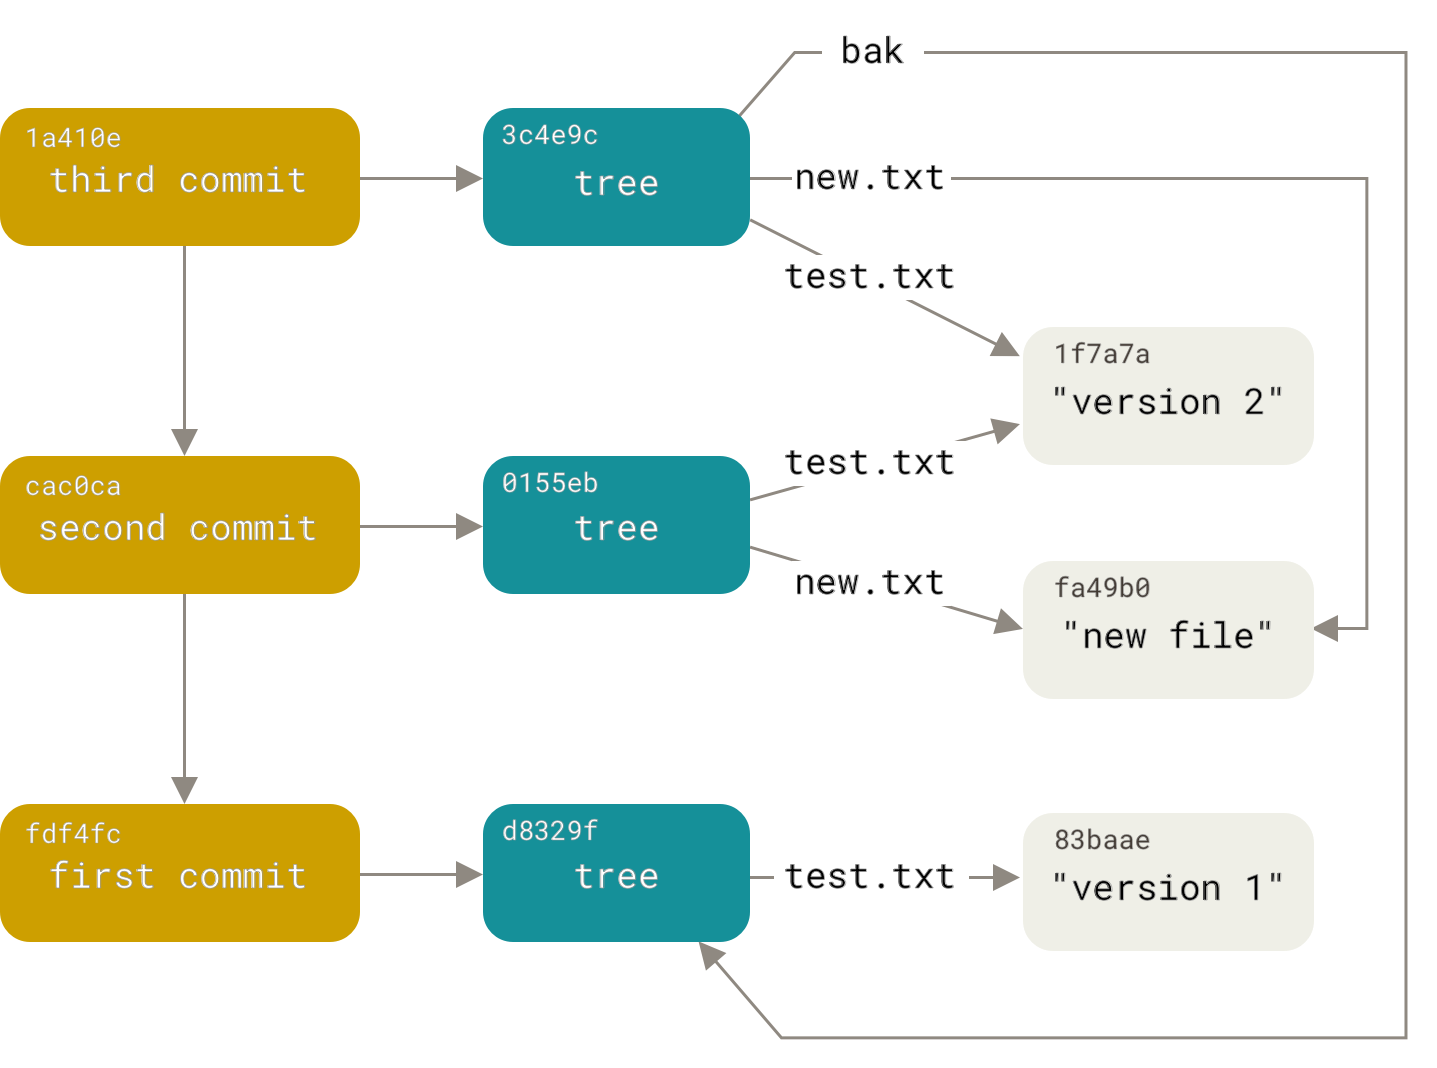
\includegraphics[width=0.8\textwidth]{./figures/vcs/git-internal-structure.png}
  \caption{Objektový model Gitu~\cite{chacon2014progit}.}
  \label{fig:git_object_model}
\end{figure}

%region Větve jako pohyblivé ukazatele
\subsection*{Větve jako pohyblivé ukazatele}
\label{subsec:git:vetve_pohyblive_ukazatele}
% CO ZDE PSÁT:
% - Dát do kontrastu s SVN (kde to byly adresářové kopie).
% - Vysvětlit, že větev v Gitu je pouhý lehký textový soubor obsahující 40 znaků (hash commitu).
% - Zmínit soubor HEAD, který určuje, na jaké větvi se uživatel právě nachází.
Dřívější \VCS{}, jako například \SVN{}, přistupovaly k~větvím jako k~fyzickým kopiím dat. To znamená, že pro vytvoření nové větve bylo nutné zkopírovat celý projekt do nové složky, což bylo prostorově i~časově náročné~\cite{chacon2014progit}.

V~Gitu jsou naproti tomu větve pouze pohyblivé ukazatele směřující na konkrétní commit. Fyzicky se jedná o~jeden textový soubor ve složce \code{.git/refs/heads/}, který obsahuje pouze hash commitu. Vytvoření větve tedy fyzicky znamená vytvoření nového souboru s~hashem commitu, což je velice rychlé bez ohledu na velikost projektu~\cite{chacon2014progit}.

Aby Git dokázal určit, na jaké větvi se uživatel právě nachází, využívá speciální ukazatel zvaný HEAD. Tento ukazatel je textový soubor uložen v~\code{.git/HEAD}, který namísto přímého hashe obsahuje symbolickou referenci na aktuální větev. Když uživatel vytvoří nový commit, Git přečte HEAD, zjistí aktuální větev a~posune její ukazatel tak, aby odkazoval na nově vzniklý commit~\cite{chacon2014progit}.

%endregion

%region Údržba a komprese dat
\subsection*{Údržba a komprese dat} % (Volitelné, ale pro akademický text vhodné)
\label{subsec:git:udrzba_komprese_dat}
% CO ZDE PSÁT:
% - Zodpovědět otázku: "Když Git ukládá celé snímky, proč repozitář nezabírá terabyty?"
% - Zmínit Garbage Collection (git gc) a Packfiles (zabalení starých objektů a použití delta komprese).
Se skutečností, že Git při každém commitu ukládá celé snímky projektu jako plné bloby, může vyvstat otázka ohledně celkové velikosti repozitáře. Git proto rozlišuje dva způsoby uložení objektů: volné objekty (loose objects) pro nově vzniklé objekty a~zabalené objekty (packed objects) pro dlouhodobé úložiště~\cite{chacon2014progit}.

Při běžné práci je každý objekt zkomprimován pomocí knihovny zlib a~uložen jako samostatný volný objekt. Liší se pouze metadata o~tom, o~jaký typ objektu se jedná~\cite{chacon2014progit}.

Když počet volných objektů překročí určitou mez, Git automaticky spustí údržbu. Během ní jsou všechny volné objekty zabaleny do jednoho velkého binárního souboru zvaného packfile. Tato operace se většinou spouští automaticky na pozadí při příkazu \code{git push} nebo ji lze vyvolat ručně příkazem \code{git gc}~\cite{chacon2014progit}.

Při vytváření packfilu je využívána delta komprese. U~tohoto způsobu komprese je nejnovější verze souboru uložena v~plném rozsahu a~všechny předchozí verze jsou uchovávány jako seznam změn vůči nejnovější verzi. Tím je zajištěn rychlý přístup k~posledním změnám, které uživatel nejčastěji potřebuje, zatímco méně využívaná historie se dopočítává, a~zároveň se výrazně zmenší celková velikost databáze~\cite{chacon2014progit}.

%endregion

%region Programovatelný přístup ke Gitu
\subsection{Programovatelný přístup ke Gitu}
\label{sec:git_api}
Programovatelný přístup ke Gitu je zajištěn pomocí knihovny \devTool{libgit2}{https://libgit2.org/}. Jedná se o~knihovnu napsanou v~jazyce C bez jakýchkoli externích závislostí, se zaměřením na programátorsky přívětivé \API{}.
Knihovna poskytuje také tzv. language bindings pro různé jazyky, včetně Rustu, Pythonu, Ruby a~dalších~\todo{Doplnit citaci}. Díky tomu je možné využívat Git pohodlně v~ostatních aplikacích bez nutnosti znalosti jazyka C.

Jedna z~nejzajímavějších vlastností této knihovny je podpora tzv. backendů (pluginů). Libgit2 umožňuje vývojářům napojit vlastní úložiště pro různé typy operací a~vytvářet vlastní pravidla pro konfiguraci, ukládání referencí nebo i~pro databázi objektů~\todo{Doplnit citaci}.

%endregion

%endregion
\endinput